\documentclass[10pt,a4paper]{article}
\setlength{\columnseprule}{0.1pt}
\setlength{\columnsep}{1cm}
\pagenumbering{gobble}
\usepackage{StileFormulario}
\renewcommand{\arraystretch}{1.15}

\newcommand{\de}{{\ensuremath{ \mbox{d}}}}
\newcommand{\norm}[1]{{\ensuremath{||{#1}||}}}
\newcommand{\ang}[1]{{\ensuremath{\langle {#1}\rangle}}}
\newcommand{\dpar}[2]{{\ensuremath{\frac{\partial {#1}}{\partial {#2}}}}}
\newcommand{\Lusc}{{\ensuremath{L^{\vec{}}}}}

\newcommand{\Pa}{ \text{ Pa} }
\renewcommand{\bar}{ \text{ bar}}
\newcommand{\atm}{ \text{ atm}}
\newcommand{\Kg}{ \text{ Kg} }
\newcommand{\m}{ \text{ m} }
\newcommand{\N}{ \text{ N} }
\newcommand{\C}{ \text{ C} }
\newcommand{\J}{ \text{ J} }
\renewcommand{\cal}{ \text{ cal} }
\newcommand{\mol}{ \text{ mol} }
\newcommand{\K}{ \text{ K} }

\title{Formulario di Fisica 3}
\date{}
\author{}

\begin{document}
\maketitle

  {\bf Disclaimer}: In classe pare usi $L_\text{entrante}=L$: è positivo se comprimo il gas.
  A volte compare $L_{uscente}=\Lusc=-L$.
  
  \section{Termodinamica}
  {\vskip 1em \large\bf Tavola delle costanti}\vskip 0.5em
  \begin{tabular}{lll}
    $R$       & $8,31 \frac{\J}{\mol \K}$                                 & costante universale dei gas \\
    $N_A$     & $6,022 \cdot 10^{23} \frac{1}{\mol}$                      & numero di Avogadro          \\
    $k = k_B$ & $k_B = \frac{R}{N_A} = 1,38 \cdot 10^{-23} \frac{\J}{\K}$ & costante di Boltzmann       \\
  \end{tabular}

  \vskip 1.5em
  \begin{tabular}{lll}
    {\bf Simbolo} &                                    & {\bf Unità di Misura}                  \\
    $p$           & pressione                          & $1 \Pa = 1 \frac{\N}{\m^2}$            \\
    $V$           & volume                             &                                        \\
    $n$           & numero di moli                     & $n = \frac{N}{N_A}$                    \\
    $T$           & temperatura assoluta               & $K$                                    \\
    $C_V$         & calore molare a volume costante    & {\it SOLO PER I GAS, NON PER I SOLIDI} \\
    $C_P$         & calore molare a pressione costante &                                        \\
  \end{tabular}

{\vskip 4em}
  
\begin{multicols}{2}
  \begin{formula}[Conversioni di unità di misure]
    1 \bar = 100 000 \Pa     \\
    1 \atm = 1,013 \bar      \\
    273,15 \K = 0 \degree \C \\
    1 \cal = 4,186 \J        \\
  \end{formula}
  
\textbf{Variabili termodinamiche}\\
Dato un sistema descritto da delle variabili termodinamiche.
Date $n$ sostanze in $f$ fasi, occorrono $2+n-f$ variabili indipendenti per descrivere il sistema, che chiameremo {\it variabili termodinamiche indipendenti}.

Molto spesso useremo un gas ($f=1$) omogeneo ($n=1$), per cui necessitiamo di $2$ variabili termodinamiche indipendenti, per esempio $(p,V)$ oppure $(T,p)$. (oppure forse $(S,T)$, non sappiamo che vuol dire).

Quindi si ha che le variabili termodinamiche sono legate tra loro da alcune equazioni, dette equazioni di stato.

In pratica, se $(p,V,T)$ descrivono il sistema, deve esistere una equazione che le lega, quindi $F(p,V,T)=0$. L'espressione di $F$ è data a priori e dipende dal sistema.

Una funzione di stato è una funzione che dipende dalle variabili termodinamiche del sistema. Esempi: Entropia $S$ e Energia Interna $U$.

Quando la funzione di stato è $F(p,V,T)$ si può spesso ricavare una variabile in funzione delle altre e quindi una volta scritta $p(v,T)= cost$ con il Teorema del Dini si ricavano le relazioni tra le derivate. (In particolare vale che il prodotto ciclico è $-1$.)

In generale, nel calcolare la quantità $\frac{\partial x}{\partial y}$ supporremo fissata la quantità $z$, dove $x,y,z$ sono le nostre variabili termodinamiche.

\begin{formula}[Coefficienti]
\text{coefficiente di espansione volumica:}\\
\beta=\frac{1}{V} \left( \frac{\partial V}{\partial T} \right)_{p fisso} \\
\text{coefficiente di compressibilità isoterma:}\\
\kappa=-\frac{1}{V} \left( \frac{\partial V}{\partial p} \right)_{T fisso}

\end{formula}
\begin{formula}[Relazioni di Maxwell per gas omogeneo]
\text{anche qua l'altra variabile è fissata}\\
\frac{\partial T}{\partial p}=\frac{\kappa}{\beta} \quad
\frac{\partial T}{\partial V}=\frac{1}{\beta V} \\
\frac{\partial p}{\partial T}=\frac{\beta}{\kappa} \quad
\frac{\partial p}{\partial V}=-\frac{1}{\kappa V}\\
\frac{\partial V}{\partial T}=\beta V \quad
\frac{\partial V}{\partial p}=-\kappa V
\end{formula}
  
\begin{formula}[Lavoro su un solido]
 \de T=0 \\
 L=-\int p \de V \\
 \de V= - \kappa V \de P \\
 L=\int^{p_2}_{p_1} \kappa V p \de p \cong \frac{\kappa V}{2} (p_2^2 -p_1^2)
\end{formula}
  
  
  \begin{formula}[Primo principio della Termodinamica]
  \text{rappresenta la conservazione dell'energia}\\
  \text{definisco il calore in questo modo} \\
    \de U = \delta Q + \delta L \\
    L =- \int p \de V  \\
  \end{formula}

Per equazioni di stato generiche non è chiaro come calcolare $U$ oppure $\delta Q$. \\
Vorremmo definire la capacità termica $C=\frac{\delta Q}{\de T}$, ma questa dipende dalla trasformazione. Se riscaldiamo a volume costante otteniamo $C=C_V$, se riscaldiamo a pressione costante otteniamo $C=C_p$.

\begin{formula}[Capacità termica]
  C_V = \dpar{U}{T}\\
  \text{$C_V$ è la capacità termica a volume costante}\\
  
  C_p= C_V + \left[ \dpar{U}{V} + p \right] V \beta \\
  \text{$C_p$ è la capacità termica a pressione costante}\\
\end{formula}

Queste formule sono utili quando ci viene data una qualsiasi equazione di stato e qualsiasi energia interna. Nel caso generale $C_V$ e $C_p$ possono non essere costanti, tipicamente dipendono dalla temperatura. Nel caso dei gas perfetti sono costanti.

\textbf{Principio zero della termodinamica} \\
Se $A$ è in equilibrio con $B$ e $B$ è in equilibrio con $C$ allora $A$ è in equilibrio con $C$.
In cui con equilibrio termodinamico si intender equilibrio termico, meccanico, chimico, ecc.

\textbf{Secondo principio termodinamica} \\
Enunciato secondo \textbf{Kelvin-Planck}: è impossibile costruire una macchina termica che, operando in un ciclo, produca il solo effetto di convertire calore in un equivalente quantitativo di lavoro.

Enunciato secondo \textbf{Clausius}: è impossibile costruire una macchina frigorifera che, operando in un ciclo, produca il solo effetto di trasferire calore da una sorgente a temperatura più bassa a una a temperature più alta.

Enunciato secondo \textbf{Carnot}: L'efficiennza di un Ciclo di Carnot reversibile dipende solo dalle temperature delle due sorgenti tra cui opera. Un macchina di Carnot rappresenta una tra le macchine termiche più efficiente tra quelle operanti tra sorgenti a temperature fissate. (A volte detto Teorema di Carnot)

Enunciato secondo \textbf{Caratheodory}: Per ogni condizione iniziale $(p,V,T)$ e per ogni intorno (di $\bbR^3$) di questa condizione esiste un punto non raggiungibile dal punto iniziale tramite una trasformazione adiabatica reversibile. Questo è equivalente a $\delta Q= T dS$.

Enunciato "moderno": In un sistema isolato vale $\frac{\de S}{\de t} \ge 0$, $t$ è il tempo. Ovvero, per un sistema termicamente isolato l'entropia non può mai diminuire e resta costante se e solo se tutte le trasformazioni sono reversibili. Si ha quindi che per qualsiasi trasformazione vale $\Delta S\ge0$. (è conseguenza della diseguaglianza di Clausius)


\textbf{Trasformazione termodinamica reversibile} \\
Una trasformazione termodinamica reversibile è una successione di trasformazioni infinitesime che passa istante per istante per degli stati di equilibrio e tale che la trasformazione inversa riporti il sistema e anche l'esterno nello stato iniziale.
In pratica si può disegnare sul piano $(V,p)$.

Esiste una trasformazione quasi-statica ma non reversibile.

\textbf{Entropia} \\
Come conseguenza del secondo principio si ha che $$ _{_{_R}} \oint \frac{\delta Q}{T}=0$$. \\
In cui con la $R$ si intende che l'integrale è calcolato lungo una trasformazione reversibile, ovvero lungo un cammino sul piano $(V,p)$.
Quindi si può definire una funzione di stato $S$ tale che per ogni coppia di stati $A$ e $B$ valga $$S(B)-S(A)= _{_{_R}}\int_{A\rightarrow B}  \frac{\delta Q}{T}$$




  \begin{formula}[Energia Interna per i gas perfetti]
    U = \frac{\ell}{2}nRT = n c_V T=C_V T
  \end{formula}

  \begin{itemize}
  \item Gas Monoatomici: $\ell =3$.
  \item Gas Biatomici: $\ell =5$.
  \item Solidi: $\ell =6$.
  \end{itemize}

  \begin{formula}[Equazione di Stato dei gas Perfetti]
    pV = nRT = NkT
  \end{formula}

  \begin{formula}[Relazione di Mayer]
    c_p - c_V = R              \\
    \gamma = \frac{c_p}{c_V}   \\
    \frac{R}{c_V} = \gamma - 1 \\
  \end{formula}
  $c_p$ è la capacità termica molare a pressione costante, anche detto calore molare a pressione costante, ovvero $\frac{C_p}{n}$, in cui $n$ è il numero di moli. $c_V$ è analogo.

  \begin{formula}[Leggi per trasformazione generica, per gas perfetti]
    \Delta U = Q - \Lusc                                                                      \\
    U = n c_V T = \frac{1}{\gamma -1} nRT                                                          \\
    \Delta S = nc_V \log \left( \frac{T_2}{T_1} \right) + n R \log \left( \frac{V_2}{V_1} \right)  \\
    \Delta S = n c_p \log \left( \frac{T_2}{T_1} \right) - n R \log \left( \frac{p_2}{p_1} \right) \\
  \end{formula}
  
  \begin{formula}[Isobara ($p$ costante)]
    \Delta U = n c_V \Delta T                            \\
    Q = n c_p \Delta T                                   \\
    \Lusc = nR \Delta T = p \Delta V                \\
    \Delta S = n c_p \log \left( \frac{T_2}{T_1} \right) \\
  \end{formula}
	
  \begin{formula}[Isoterma ($T$ costante)]
    \Delta U = 0 \implies Q = \Lusc                 \\
    Q = nRT \log \left( \frac{V_2}{V_1} \right)          \\
    \Lusc = nRT \log \left( \frac{V_2}{V_1} \right) \\
    \Delta S = nR \log \left( \frac{V_2}{V_1} \right)    \\
  \end{formula}

  \begin{formula}[Isocora ($V$ costante)]
    \Delta U = n c_V \Delta T                            \\
    Q = n c_V \Delta T                                   \\
    \Lusc = 0                                       \\
    \Delta S = n c_V \log \left( \frac{T_2}{T_1} \right) \\
  \end{formula}

  \begin{formula}[Adiabatica reversibile senza scambio di calore]
    \Delta U = n c_V \Delta T                                          \\
    Q = 0                                                              \\
    \Lusc = \Delta U = n c_V \Delta T = \frac{\Delta (pV)}{1 - \gamma} \\
    pV^\gamma = \text{cost}                                            \\
    TV^{\gamma -1} = \text{cost}                                       \\
    pT^{\frac{\gamma}{1-\gamma}} = \text{cost}                         \\
    \text{l'entropia non varia, verificare}
  \end{formula}
  
 
  \textbf{ Espansione libera} \\
  In generale vale $$\delta Q=0, \delta L=0 \Rightarrow U=cost$$
  Nel caso dei gas perfetti, per definizione, vale $\de T=0$, cioè la temperatura, e quindi l'energia interna, non cambia.
  $\Delta U=0$. \\
  Per calcolare la variazione di entropia non posso usare la formula $\int_{A\rightarrow B} \frac{\delta Q}{T}$ calcolata lungo l'espansione libera (infatti l'integrale fa $0$, poiché $\de Q=0$) poiché non è reversibile. Prendo quindi un'isoterma (reversibile!) che passa per il punto iniziale e finale si calcola che $\Delta S = nR \log \left( \frac{V_2}{V_1} \right)$


  \begin{formula}[Relazioni sui differenziali, gas perfetto]
    \de{U} + \delta \Lusc = \delta{Q}                                   \\
    pV = nRT \implies p\de{V} + V\de{p} = nR\de{T}                      \\
    \delta \Lusc  = p\de{V},                                          \\
    \de{U} = nc_V \de{T}                                                \\
    \de{U} \frac{R}{c_V} = nR\de{T} = \delta \Lusc + V\de{p} =       \\
    = \delta {Q} - \de{U} + V\de{p} \implies \delta {Q} = nc_p \de{T} - V\de{p} \\
    \text{Vale anche:}\\
    \delta Q= \de U - \delta L= C_V \de T + p \de V
  \end{formula}

  \begin{formula}[Legge di Van der Waals]
    (p+a\frac{n^2}{V^2})(V-nb) = nRT
  \end{formula}



  {\bf Fatti casuali}
  \begin{itemize}
  \item Entropia per i Gas Perfetti: $S = nc_V \log T + nR \log \frac{V}{n}$
  \item Calore assorbito (per i non-gas): $\mbox{d}Q = c m \mbox{d}T$, con $c$ calore specifico del corpo.
  \item Entropia: $T \mbox{d}S = \mbox{d}U + p \mbox{d}V$, $\mbox{d}S = \left(\frac{\mbox{d}Q}{T}\right)_{\mbox{reversibile}}$
  \item Calore assorbito (per i gas): $\mbox{d}Q = n c_V \mbox{d}T$, con $c_V$ capacità termica molare a volume costante, anche detto calore molare a pressione costante. Attento che può dipendere dal libro.
  \item Energia libera (o potenziale di Helmholz): $F = U - TS$
  \item Entalpia: $H = U + pV$.
  \item Energia libera di Gibbs: $G = U + pV - TS=H-TS=F+pV$
  \end{itemize}

  \begin{itemize}
  \item Capacità Termica di un corpo: $C = \frac{\Delta Q}{\Delta T}$
  \item Conduzione: $\frac{Q}{\Delta t} = \frac{k A \Delta T}{d}$; $k$ conducibilit\`a termica, $A$ Area, $d$ spessore parete.
  \item Irraggiamento: $\frac{\de E}{\de t} = \varepsilon \sigma A (\Delta T^4)$, $\varepsilon$ emissivit\`a, $\sigma$ costante di Stefan-Boltzmann.
  \end{itemize}

\textbf{Potenziali termodinamici e condizioni di equilibrio} \\
$\Delta F$, $\Delta H$, $\Delta H < 0$ per trasformazioni spontanee. DA FARE, vedi Picasso. \\

Su una trasformazione reversibile vale che $\de F = - p \de V - S \de T$ e quindi se riusciamo ad esprimere $F$ come funzione della coppia $(V, T)$, si ottiene $p = - \lrt{\dpar{F}{V}}_T$ (a temperatura costante) e anche $S = - \lrt{\dpar{F}{T}}_V$.

\textbf{Significato microscopico dell'entropia} \\
$S=k_B ln \Omega$. DA FARE, vedi Picasso. \\

\textbf{Ciclo di Carnot} \\
Compressione Adiabatica, Espansione Isoterma, Espansione Adiabatica, Compressione Isoterma. \\
Compressione $=$ volume diminuisce (dal latino comprimére). \\
$\eta = 1- \frac{T_L}{T_H}$

\textbf{Ciclo di Stirling} \\
Isocora ($p$ aumenta), Espansione Isoterma, Isocora ($p$ diminuisce), Compressione Isoterma. \\
$\eta = 1- \frac{T_L}{T_H}$

\textbf{Ciclo Otto, Gasoline} \\
Isocora ($p$ aumenta) (da $T_2$ a $T_3$), Espansione adiabatica, Isocora ($p$ diminuisce), Compressione Isocora. \\
$\eta = 1- \frac{T_1}{T_2}$ (da Wikipedia, Il Picasso NON è d'accordo, da controllare)

\textbf{Ciclo Diesel} \\
Compressione adiabatica (da $T_1$ a $T_2$), Espansione Isobara, Espansione Adiabatica, Isobara ($p$ diminuisce). \\
$\eta= 1-\frac{1}{\gamma} \frac{r^\gamma -1}{r-1} \frac{T_1}{T_2}$ \\
$r=\frac{V_1}{V_3}$, $\gamma$ è quello delle relazioni di Mayer.


\textbf{Rendimento di un ciclo generico} \\
Posso sempre interpretare un ciclo reversibile come una macchina termica che opera tra infinite sorgenti, una per ogni temperatura raggiunta dal sistema durante il ciclo. Questa è un'ipotesi necessaria affinché il ciclo sia reversibile. 
Geometricamente ciò corrisponde a sezionare il ciclo con delle isoterme. 
Operativamente per calcolare il rendimento si calcola il calore netto $\delta Q(T)$ scambiato con ogni sorgente $T$. Definiamo poi $Q_{ass}=\sum_T \max\{ \delta Q(T), 0 \}$, in pratica sommiamo, sorgente per sorgente, solo i calori che entrano nella macchina.
Il lavoro è l'area racchiusa dalla curva.
  
A seconda del verso di percorrenza un ciclo può essere una macchina termica o una macchina frigorifera (dal segno del lavoro $\Lusc$). Pompa di calore è un altro nome per macchina frigorifera.
  \begin{itemize}
  \item Rendimento di una macchina termica: $\eta = \frac{\Lusc}{Q_{ass}}$
  \item Efficienza di un macchina frigorifera: $\epsilon = \mbox{COP}_f= \frac{Q_{\mbox{tolto al frigo}}}{L}$
  \item Efficienza di una pompa di calore: $\mbox{COP}_{pc}= \frac{Q_{\mbox{dato alla sorgente calda}}}{L}$ (stesso disegno di una macchina frigorifera)
  \end{itemize}

  \subsection*{``Approfondimento''}
  \begin{itemize}
  \item Equazione di Clapeyron: descrive la variazione della pressione con la temperatura della curva di equilibrio (di solito si pensa nel piano $(T,p)$) tra due fasi di una stessa sostanza (è una curva per la regola delle fasi: $n=1$, $f=2$): $$\frac{\de p}{\de T} =\frac{\lambda}{T (v_B - v_A)}$$. \\
  $\lambda$ è il calore latente (per unità di massa) di transizione a una fase all'altra. \\
  $v$ è il volume specifico delle due fasi $A$ e $B$. (il volume specifico è volume diviso massa, quindi l'inverso della densità volumica)
  \item Legge di Dalton: "In una miscela di gas la pressione totale \`e uguale alla somma delle pressioni parziali dei suoi gas componenti". $$P_{TOT} = \frac{RT}{V}\left( \sum_{i} n_i \right)$$
  \item Forza media che {\bf una} molecola esercita sul contenitore cubico di lato $L$: $\norm{\vec{F}} = \frac{mv^2}{L}$
  \item Forza totale esercitata dal gas: $\norm{\vec{F}} = \frac{1}{3}N \left(\frac{m \ang{v^2}}{L} \right)$, con $\ang{v^2}$ valor medio del quadrato della velocit\`a. $v_{qm} := (\ang{v^2})^{\frac{1}{2}}$ \`e la velocit\`a quadratica media.
  \item $P = \frac{\norm{\vec{F_{TOT}}}}{L^2} = \frac{2}{3} N \left(\frac{1}{2}m {v_{qm}^{2}} \right) \frac{1}{V} = \frac{2}{3} N \ang{E_{cin}}$, $\ang{E_{cin}} = \frac{l}{2}K_BT = \frac{1}{2}m{v_{qm}^\frac{1}{2}}$, $l$ gradi di libert\`a.
  \end{itemize}

  \clearpage
  
  \section{Onde}
  \subsection*{Generalitate}
  \begin{tabular}{lc}
    Equazione d'onda         & $\partial_{xx} \Psi - \frac{1}{c^2} \partial_{tt} \Psi = 0$ \\
    Relazione di dispersione & $\omega^2 = c^2 k^2$                                        \\
    Numero d'onda            & $k$                                                         \\
    Periodo dell'onda        & $T = \frac{2 \pi}{\omega}$                                  \\
    Pulsazione               & $\omega = 2 \pi f$                                          \\
    Lunghezza d'onda         & $\lambda = \frac{2 \pi}{k} = cT$                            \\
    Intensità dell'onda      & $I = \abs{A}^2$                                             \\
  \end{tabular}

  \begin{paragrafo}[Forma delle onde]
    Tutte le soluzioni dell'equazione d'onda (anche detta equazione di D'Alambert) sono della forma $\Psi(x, t) = f_1(x - ct) + f_2(x + ct)$.

    Inoltre se cerchiamo di risolvere l'equazione tridimensionale $c^2 \nabla^2 \Psi = \frac{\partial^2 \Psi}{\partial t^2}$ le soluzioni saranno della forma $\Psi(x, y, z, t) = f_1(\alpha x + \beta y + \gamma z + ct) + f_1(\alpha x + \beta y + \gamma z - ct)$ con $\alpha^2 + \beta^2 + \gamma^2 = 1$

    L'analoga formula per le onde invarianti per rotazioni è $\Psi(r, t) = \frac{f_1(r - ct) + f_2(r + ct)}{r}$.
  \end{paragrafo}

  \subsection*{Formule di M. Complete}
  \begin{equation*}
    \div {\vec E} = \frac{\rho}{\epsilon_0}
  \end{equation*}
  \begin{equation*}
    \div {\vec B} = 0
  \end{equation*}
  \begin{equation*}
    \rot {\vec E} = - \dep{\vec B}{t}
  \end{equation*}
  \begin{equation*}
    \rot {\vec B} = \epsilon_0 \mu_0 \dep{\vec E}{t} + \mu_0 \vec J
  \end{equation*}

  \subsection*{Potenziali e Gauge}
  Si deve avere:
  \begin{eqsystem}[c]
    \vec E = - \grad V - \dep{\vec A}{t} \\
    \vec B = \rot {\vec A} \\
  \end{eqsystem}
  
  Nella Gauge di Lorentz, ovvero
  $\div {\vec A} + \mu_0 \epsilon_0 \dep{V}{t} = 0$, si ha
  \begin{eqsystem}[c]
    - \nabla^2 V + \frac{1}{c^2} \dep{V}{t} = \frac{\rho}{\epsilon_0} \\
    - \nabla^2 {\vec A} + \frac{1}{c^2} \dep{\vec A}{t} = \mu_0 \vec J \\
  \end{eqsystem}

  Inoltre esiste la Gauge di Coulomb $\div {\vec A} = 0$, nella quale si ottiene:
  \begin{eqsystem}[c]
    - \lapl V = \frac{\rho}{\epsilon_0} \\
    - \lapl {\vec A} + \mu_0 \epsilon_0 \dpar{^2 {\vec A}}{t^2} = + \mu_0 {\vec J} - \mu_0 \epsilon_0 \grad \lrt{\dpar{V}{t}} \\
  \end{eqsystem}
  
  \subsection*{Riflessione dell'onda}
  \begin{center}
    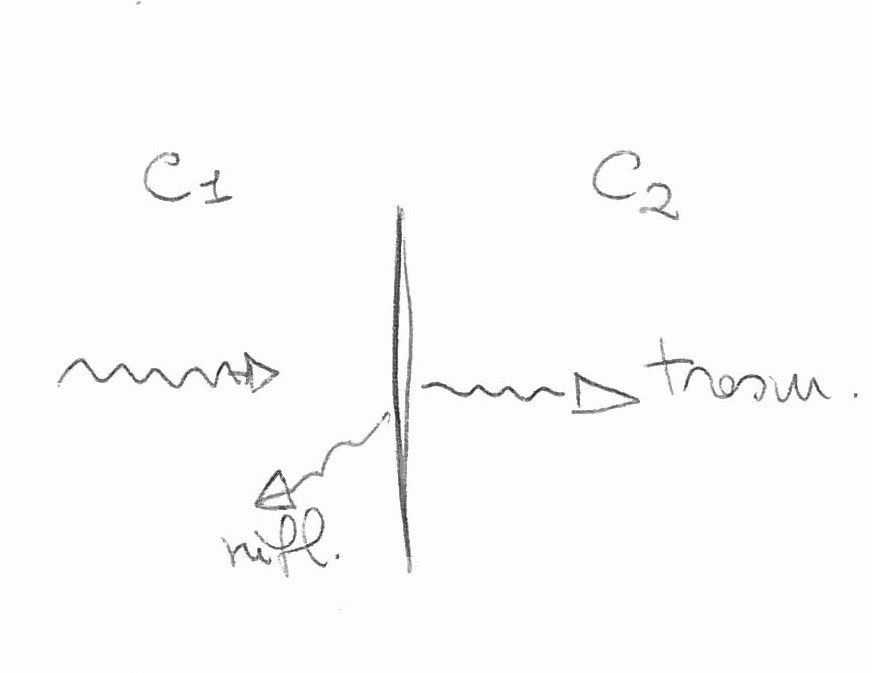
\includegraphics[width=0.65\linewidth]{riflessione-onde}
  \end{center}
  
  \begin{paragrafo}[Problema della Riflessione]
    Ci viene data un'onda monocromatica della forma $A_1 e^{i(kx - \omega t)}$ in un mezzo con velocità della luce $c_1$, e ci viene chiesto di dire chi è l'onda trasmessa nel mezzo con velocità della luce $c_2$ e quella riflessa nel mezzo di partenza.

    I pedici nel seguito sono $1$ per l'onda nota, $T$ per l'onda trasmessa e $R$ per l'onda riflessa.
  \end{paragrafo}
  
  $$ \Psi(x, t) = \left\{
    \begin{array}{lr}
      \Psi_1(x, t) & x < 0 \\
      \Psi_2(x, t) & x > 0 \\
    \end{array}
  \right. $$

  \begin{tabular}{lcl}
    $\Psi_1(x, t)$ & = & $A_1 e^{i(kx - \omega t)} + A_R e^{i(k_R x - \omega t)}$ \\
    $\Psi_2(x, t)$ & = & $A_T e^{i(k_T x - \omega t)}$                            \\
  \end{tabular}

  dove vale che $c_2^2 k_T^2 = \omega^2 = c_1^2 k^2 = c_1^2 k_R^2$ e quindi abbiamo le relazioni $k_R = - k$ (perché è riflessa), $k_T = \frac{c_1}{c_2} k$.

  Imponendo il raccordo $\cC^0$ con $\Psi_1(0, t) = \Psi_2(0, t)$ si ottiene $A_1 + A_R = A_T$.
  
  Imponendo il raccordo $\cC^1$ con $\partial_x \Psi_1(0, t) = \partial_x \Psi_2(0, t)$ si ottiene $k A_1 + k_R A_R = k_T A_T$.

  e quindi risolvendo $A_T = \frac{2 c_2}{c_1 + c_2} A_1$, $A_R = \frac{c_2 - c_1}{c_1 + c_2} A_1$.                      

  \subsection*{Interferenza tra due sorgenti}
  \begin{center}
    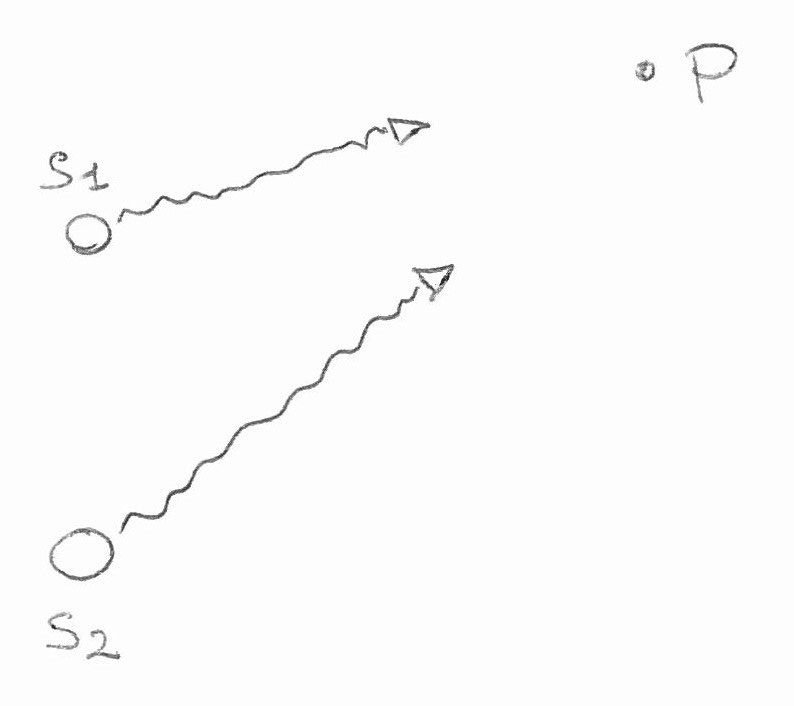
\includegraphics[width=0.65\linewidth]{interferenza-sorgenti}
  \end{center}

  \begin{paragrafo}[Problema dell'interferenza]
    Abbiamo due sorgenti uguali (stesso $\omega$ e stesso $k$) che emettono onde sferiche monocromatiche (in notazione complessa $\frac{e^{-i\omega t - ikr}}{r}$, dove $r$ è la distanza dalla sorgente). Ci mettiamo in un punto $P$ e calcoliamo l'intensità con cui le onde arrivano in $P$.
  \end{paragrafo}

  Allora se scriviamo l'onda che arriva nel punto $P$ da ciascuna sorgente $\Psi_i = \Psi_0 \frac{\cos(k r_i - \omega t)}{r_i}$ per $i = 1, 2$, possiamo calcolare l'intensità dell'onda e si ha che
  $$ I = \frac{\Psi_0^2}{r_1^2} + \frac{\Psi_0^2}{r_2^2} + 2 \frac{\Psi_0^2}{r_1 r_2} \cos \delta $$
  dove $\delta = k (r_2 - r_1)$

  Inoltre, se $\cos \delta = 1$ diciamo che nel punto si ha interferenza {\it costruttiva}, se $\cos \delta = -1$ diciamo che nel punto si ha interferenza {\it distruttiva}.

  {\bf Approssimazione a grande distanza}
  Supponiamo che $r_1 \approx r_2 = r$ e che $r >> d$ (con $d$ indichiamo la distanza tra le due sorgenti). Indichiamo inoltre con $\theta$ l'angolo tra il punto $P$ e la retta dei punti equidistanti dalle due sorgenti. Allora si ha che $r_2 - r_1 \approx d \sin\theta$ e la formula dell'intensità si esprime come
  $$ I = \frac{4 \Psi_0^2}{r^2} \cos^2 \lrt{\frac{\delta}{2}} = \frac{4 \Psi_0^2}{r^2} \cos^2 \lrt{\frac{\pi d}{\lambda} \sin\theta} $$

  \begin{formula}[Equazioni nel vuoto]
    \square = \nabla^2 - \frac{1}{c^2} \frac{\partial^2}{\partial t^2} \\
    \text{Allora le equazioni nel vuoto diventano} \\
    \square {\vec B} = 0, \hskip 1.5em \square {\vec E} = 0
  \end{formula}

  \subsection*{Formula Onda Piana nel vuoto, Polarizzazione lineare}
  \begin{eqsystem}[rl]
    \vec E = & \vec{E_0} \cos (\vec{k} \dotp \vec{r} - \omega t + \varphi_0) \\
    \vec B = & \vec{B_0} \cos (\vec{K} \dotp \vec{r} - \omega t + \varphi_0) \\
  \end{eqsystem}
  con $\vec{B_0} = \frac{1}{c} \hat{k} \times \vec{E}$ e $\omega = ck$.

  \subsection*{Formula Onda Piana nel vuoto, Polarizzazione circolare}
  \begin{eqsystem}[rl]
    \vec E = & (\vec{a_0} \pm i \hat{k} \times \vec{a_0}) e^{i (\vec{k} \dotp \vec{r} - \omega t + \varphi_0)}             \\
    \vec B = & \frac{1}{c} (\hat{k} \times \vec{a_0} \mp i \vec{a_0}) e^{i (\vec{k} \dotp \vec{r} - \omega t + \varphi_0)} \\
  \end{eqsystem}

  \subsection*{Formula Onde Sferiche nel Vuoto}
  \begin{eqsystem}[rl]
    \vec E = & \frac{E_0}{r} e^{i ({\vec k} \dotp {\vec r} \pm \omega t + \varphi_0)} \hat{r} \\
    \vec B = & \frac{B_0}{r} e^{i ({\vec k} \dotp {\vec r} \pm \omega t + \varphi_0)} \hat{r} \\
  \end{eqsystem}
    
  Chiamiamo vettore di Poynting
  $\vec{I} = \frac{1}{\mu_0} (\vec{E} \times \vec{B})$, siccome si ha,
  fissato un volume $V$, e detta $\Sigma = \partial V$ il suo bordo:
  $$\frac{\de}{\de t} \lrt{\int_{V_\epsilon} u_E + u_B} = -
  \frac{1}{\mu_0} \int_\Sigma (\vec{E} \times \vec{B}) \dotp \de{\vec{s}}$$
    
  E la densità di quantità di moto $\vec P = \frac{1}{c} \vec S$. Densità di momento angolare $\vec{m_\Omega} = (\vec r - \vec \Omega) \times \vec{P}(\vec r)$
  
  \begin{paragrafo}[Riflessione di un onda]
    $\vec E = \vec{E_+} + \vec{E_-}$ ed
    anche $\vec B = \vec{B_+} + \vec{B_-}$, dove con il $+$ indichiamo i
    campi incidenti e con il $-$ indichiamo i campi riflessi.
    
    % TODO: Da finire
    
    Ricordiamo che per le onde piane si ha $\vec{\nabla} = i \vec{k}$, ovvero $\rot (e^{\vec k \cdot \vec r} \vec u) = (i \vec{k} \times u) e^{\vec k \cdot \vec r}$ e simili.
  \end{paragrafo}
  
  \begin{paragrafo}[Velocità della luce in un mezzo]
    $v = \frac{c}{\sqrt{\epsilon_r \mu_r}}$ è la velocità della luce.
    
    Inoltre $n_r = \frac{v}{c}$ si dice indice di rifrazione
  \end{paragrafo}
  
  \begin{paragrafo}[Onde incidenti, rifratte, riflesse]
    \begin{center}
      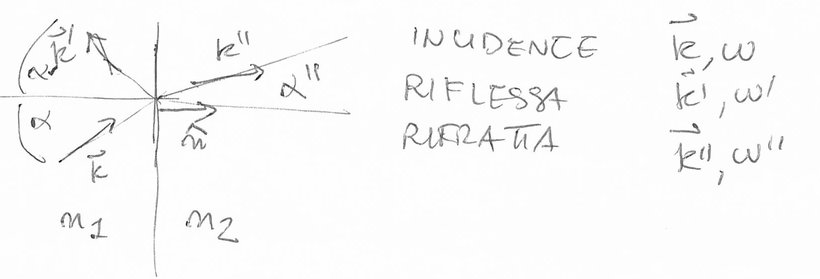
\includegraphics[width=0.95\linewidth]{onde-riflesse-rifratte}
    \end{center}
    
    Imponendo la continuità dei campi nei materiali si ottiene $\omega =
    \omega' = \omega''$, $\alpha = \alpha'$, ovvero che l'angolo di
    riflessione è uguale all'angolo di incidenza.
    
    Inoltre per la relazione di snell
    $n_2 \sin \alpha'' = n_1 \sin \alpha$
    
    Se la polarizzazione è ortogonale sia a $\hat{k}$ sia a $\hat{n}$,
    vale che
    \begin{displaymath}
      \begin{array}{c}
        E_0' = \frac{n_1 \cos \alpha - n_2 \cos \alpha'}{n_1 \cos \alpha + n_2 \cos \alpha''} \\
        E_0'' = E_0 \frac{2 n_1 \cos \alpha}{n_1 \cos \alpha + n_2 \cos \alpha'}              \\
      \end{array}
    \end{displaymath}
  \end{paragrafo}
  
  \begin{paragrafo}[Potenziali ritardati]
    \begin{eqsystem}[rl]
      V =       & \frac{1}{4 \pi \epsilon_0} \int \frac{\rho(\vec{r}', t - \frac{\abs{\vec{r} - \vec{r}'}}{c})}{\abs{\vec{r} - \vec{r}'}} \de^3 r' \\
      \vec{A} = & \frac{\mu_0}{4 \pi} \int \frac{\vec{J}(\vec{r}', t - \frac{\abs{\vec{r} - \vec{r}'}}{c})}{\abs{\vec{r} - \vec{r}'}} \de^3 r'     \\
    \end{eqsystem}
    Ed è soddisfatta la Gauge di Lorentz: $\div {\vec A} + \frac{1}{c^2}
    \frac{\partial^2 V}{\partial t^2} = 0$.
  \end{paragrafo}

  \subsection*{Principia Relativitatis}
  Postulati della teoria della Relatività Ristretta (o Speciale)
  \begin{itemize}
  \item La leggi della meccanica, dell'elettromagnetismo e dell'ottica sono le stesse in tutti i sistemi di riferimento inerziali
  \item La luce si propaga nel vuoto a velocità costante $c$ indipendentemente dallo stato di moto della sorgente e dell'osservatore
  \end{itemize}

  \subsection*{Velocità e Lunghezza}
  Un evento è identificato da quattro coordinate $(t, x, y, z)$.

  La distanza ``lungo x'' $L_x$ tra due eventi $(t, x_1, y_1, z_1)$ e $(t, x_2, y_2, z_2)$, simultanei in un dato sistema di riferimento $\Sigma$, è definita come $\abs{x_1 - x_2}$. La lunghezza ``lungo x'' di un oggetto unidimensionale è la distanza ``lungo x'' tra i due estremi.

  \subsection*{Rapidità}
  
  \subsection*{Formule per $\beta$ e $\gamma$}
  $\vec \beta = \frac{\vec v}{c}$, $\gamma = \frac{1}{\sqrt{1 - \beta^2}}$. Vale quindi $\beta^2 \gamma^2 = \gamma^2 - 1$. Inoltre $\gamma > 1$ e $\beta < 1$ sempre.

  Vogliamo dare una ``distanza'' tra due eventi nello spazio quadridimensionale,  $A = (c t_1, x_1, y_1, z_1)$, $B = (c t_2, x_2, y_2, z_2)$.
  \begin{formula}[Intervallo Invariante]
    S(A, B)^2 = (c t_1 - c t_2)^2 - (x_1 - x_2)^2 - (y_1 - y_2)^2 - (z_1 - z_2)^2
  \end{formula}

  \subsection*{Boost generico}
  Nel caso in cui la velocità di $\Sigma'$ scritta rispetto alle coordinate di $\Sigma$ sia $v = (v_x, v_y, v_z)$, la matrice con cui cambiano le coordinate è
  \begin{displaymath}
    \lrt{
      \begin{array}{cccc}
        \gamma & - \gamma \beta_x & - \gamma \beta_y & - \gamma \beta_z \\
        - \gamma \beta_x & 1 + (\gamma - 1) \frac{\beta_x^2}{\beta^2} & (\gamma - 1) \frac{\beta_x \beta_y}{\beta^2} & (\gamma - 1) \frac{\beta_x \beta_z}{\beta^2} \\
        - \gamma \beta_y & (\gamma - 1) \frac{\beta_y \beta_x}{\beta^2} & 1 + (\gamma - 1) \frac{\beta_y^2}{\beta^2} & (\gamma - 1) \frac{\beta_y \beta_z}{\beta^2} \\
        - \gamma \beta_z & (\gamma - 1) \frac{\beta_z \beta_x}{\beta^2} & (\gamma - 1) \frac{\beta_z \beta_y}{\beta^2} & 1 + (\gamma - 1) \frac{\beta_z^2}{\beta^2} \\
      \end{array}
    }
  \end{displaymath}
  con $(\beta_x, \beta_y, \beta_z) = \frac{1}{c} (v_x, v_y, v_z)$, di modulo $\beta$.
  
  \subsection*{Boost lungo $\hat{x}$}
  \begin{displaymath}
    \lrt{\begin{array}{c} ct' \\ x' \\ y' \\ z' \\ \end{array}} =
    \lrt{
      \begin{array}{cccc}
        \gamma & - \beta \gamma & 0 & 0 \\
        - \beta \gamma & \gamma & 0 & 0 \\
        0 & 0 & 1 & 0 \\
        0 & 0 & 0 & 1 \\
      \end{array}
    } \cdot
    \lrt{\begin{array}{c} ct \\ x \\ y \\ z \\ \end{array}}
  \end{displaymath}
  dove $\beta = \frac{v_x}{c}$ e $(v_x, 0, 0)$ è la velocità del sistema $\Sigma'$ scritta nelle coordinate del sistema $\Sigma$.

  \subsection*{Contrazione delle lunghezze}
  Prendiamo un corpo in moto, nel nostro sistema di riferimento $\Sigma_\text{lab}$, con velocità $(v_x, 0, 0)$ costante. Esiste un sistema di riferimento, detto proprio, in cui l'oggetto ha velocità nulla (è il sistema di riferimento che va a velocità $(-v_x, 0, 0)$ misurata nel sistema $\Sigma_\text{lab}$).
  $$ L_{x,\text{osservata}} = \frac{L_{x, \text{propria}}}{\gamma(v_\text{osservata})} $$
  dove le $L_x$ indicano solo la lunghezza lungo $\hat{x}$.
  
  \subsection*{Dilatazione dei tempi}
  Supponiamo di avere due eventi che in un sistema di riferimento $\Sigma$ hanno uguali coordinate spaziali.
  $$ \Delta T_\text{osservato} = \Delta T_\text{proprio} \cdot \gamma(v_\text{osservata}) $$

  \subsection*{Quadricose}
  In un sistema di riferimento fissato, definiamo le seguenti quantità:
  \begin{displaymath}
    \begin{array}{c}
      X^\mu = (ct, x, y, z) \\
      \de t = \gamma \de \tau \\
      U^\mu = \ded{X^\mu}{\tau} \\
      U^\mu = \gamma (c, v_x, v_y, v_z) \\
      P^\mu = m U^\mu = m \gamma (c, v_x, v_y, v_z) = (\frac{E}{c}, p_x, p_y, p_z) \\
      F^\mu = \ded{P^\mu}{\tau} = \gamma (\frac{1}{c} \vec{f} \dotp \vec{v}, f_x, f_y, f_z) \\
    \end{array}
  \end{displaymath}
  dove $\vec{f}$ è la forza classica e $\vec{v}$ è la velocità classica. Come caso particolare, posto $\vec p = m \gamma(v) \vec v$, vale l'equazione $\ded{\vec p}{t} = \vec f$. 

  Tutte le quantità definite sopra sono quadrivettori, ovvero trasformano con le matrici di Lorentz per cambi di sistema di riferimento.

  In particolare la quadrinorma di $P$ è costante in tutti i sistemi di riferimento inerziali e vale $\norm{P}^2 = m^2 c^2$, ovvero vale $\frac{E^2}{c^2} - {\vec p} \dotp {\vec p} = m^2 c^2$, dove $\vec p = (p_x, p_y, p_z)$.

  \subsection*{Urti}
  In una interazione tra $n$ particelle con quadrivettori energia-impulso $P_1, \ldots, P_n$, il cui risultato sono $m$ particelle con quadrivettori $Q_1, \ldots, Q_m$ vale l'uguaglianza $\sum_i P_i = \sum_j Q_j$ (come quadrivettori).

  \subsection*{Particelle a massa nulla}
  Il quadrivettore impulso per un'onda elettromagnetica (fotone) si scrive $P = \hbar (\frac{\omega}{c}, k_x, k_y, k_z)$.
  Il fatto che la massa sia nulla è equivalente alla relazione $c^2 \, \vec{k} \dotp \vec{k} = \omega^2$.
  Essendo un quadrivettore possiamo dedurre come cambia la frequenza di un'onda elettromagnetica per cambi di sistema di riferimento.

  \subsection*{Cambio di Campi}
  Per un boost lungo $\hat x$ i campi elettrico e magnetico cambiano come:
  \begin{displaymath}
    \begin{array}{cc}
      E_x' = E_x & B_x' = B_x \\
      E_y' = \gamma (E_y - \beta c B_z) & B_y' = \gamma (B_y + \beta \frac{E_z}{c}) \\
      E_z' = \gamma (E_z + \beta c B_y) & B_z' = \gamma (B_z - \beta \frac{E_y}{c}) \\
    \end{array}
  \end{displaymath}

  In generale, per un boost lungo $\vec \beta$ si hanno le formule:
  \begin{displaymath}
    \begin{array}{c}
      \vec{E'} = \gamma (\vec E + c \vec \beta \times \vec B) - \frac{\gamma^2}{\gamma + 1} \vec \beta (\vec \beta \dotp \vec E) \\
      \vec{B'} = \gamma (\vec B - \frac{1}{c} \vec \beta \times \vec E) - \frac{\gamma^2}{\gamma + 1} \vec \beta (\vec \beta \dotp \vec B) \\
    \end{array}
  \end{displaymath}

  Comunque sia le quantità $B^2 - \frac{E^2}{c^2}$ e $\vec B \dotp \vec E$ sono invarianti per cambio di sistema di riferimento.

  \subsection*{Effetto Doppler Relativistico}
  Sia $\nu_s$ la frequenza della sorgente (nel sistema di riferimento dell'osservatore) e $\nu_o$ la frequenza osservata

  \subsubsection*{Effetto Doppler Parallelo}
  $$ \nu_o = \sqrt{\frac{1 - \beta}{1 + \beta}} \nu_s $$
  Per essere sicuri del segno di $\beta$, ricordare che se la sorgente si avvicina all'osservatore, la frequenza osservata è maggiore di quella emessa.
  
  \subsubsection*{Effetto Doppler Trasverso}
  Qualora la congiungente tra l'osservatore e la sorgente (detta direzione di osservazione) sia ortogonale alla velocità della sorgente, vale la formula
  $$ \nu_o = \frac{1}{\gamma} \nu_s $$

  Nel caso generale, detto $\theta$ l'angolo tra la direzione di osservazione e la velocità della sorgente, si ha
  $$ \nu_o = \frac{\nu_s}{\gamma (1 + \frac{v}{c} \cos\theta)} $$

  \begin{center}
    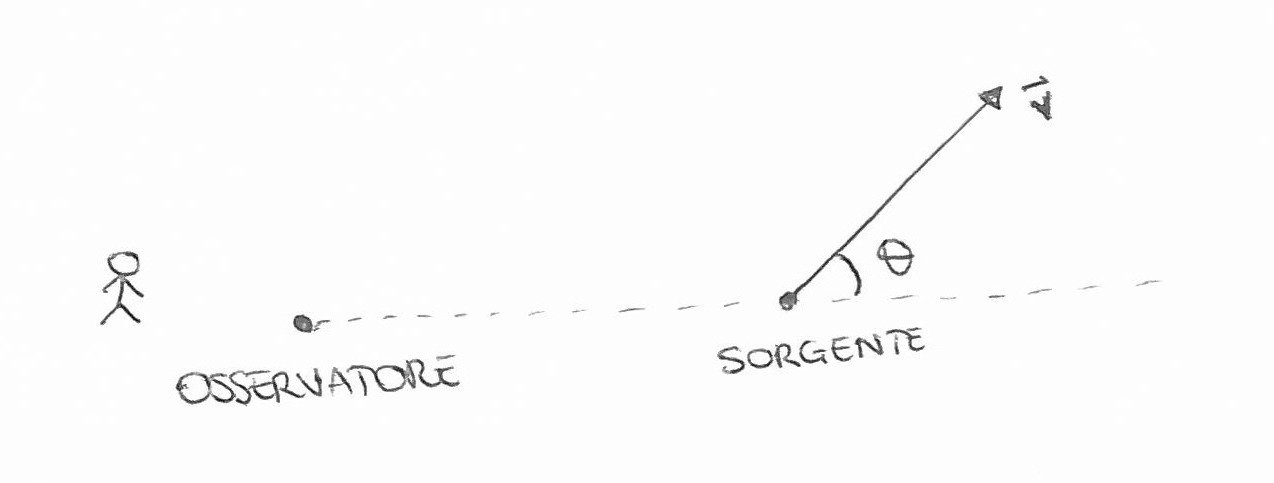
\includegraphics[width=0.85\linewidth]{osservatore-sorgente}
  \end{center}

  \subsection*{Composizione delle velocità}
  Dato un punto materiale $P$ che si muove di moto rettilineo uniforme e due sistemi di riferimento $\Sigma$ e $\Sigma'$. Detti $\vec u$ la velocità di $P$ rispetto a $\Sigma$, $\vec u'$ la velocità di $P$ rispetto a $\Sigma'$ e $\vec v$ la velocità di $\Sigma'$ rispetto a $\Sigma$, vale la seguente relazione
  $$ \vec u' = \frac{\vec u + \lrq{(\gamma_v - 1) \frac{\vec u \dotp \vec v}{v^2} - \gamma_v} \vec v}{\gamma_v \lrt{1 - \frac{\vec u \dotp \vec v}{c^2}}} $$

  In particolare, nel caso in cui si abbia $v = (v_x, 0, 0)$ valgono le seguenti formule: detto $\eta = 1 - \frac{v_x u_x}{c^2}$
  \begin{displaymath}
    \begin{array}{c}
      u_x' = \frac{1}{\eta} (u_x - v_x) \\
      u_y' = u_y (\eta \gamma_v)^{-1} \\
      u_z' = u_z (\eta \gamma_v)^{-1} \\
    \end{array}
  \end{displaymath}

  \subsection*{Calcolo del Tempo proprio}
  Supponiamo in un dato sistema di riferimento di osservare un corpo muoversi secondo una legge oraria $\vec X(t)$ con velocità $v(t)$ per $t \in [0, T]$, dove $X$ e $t$ sono le coordinate nel sistema di riferimento dell'osservatore. Allora il tempo proprio trascorso, ovvero il tempo trascorso percepito dall'oggetto, risulta essere
  $$ \tau (T) = \int_0^T \frac{\de t}{\gamma(v(t))} $$

  \subsection*{Rapidità}
  La rapidità è una funzione della velocità definita come
  $$ w(v) = \text{settanh} \lrt{\frac{v}{c}} $$
  Nella composizione delle velocità, le rapidità si sommano.

  \subsection*{Pacchetti d'onda e velocità di gruppo}
  Supponiamo di avere un mezzo in cui la velocità di propagazione di un'impulso dipende dalla frequenza dell'impulso stesso. Operativamente significa che l'impulso si scrive
  $$ \phi(x, t) = \int_{-\infty}^{\infty} A(k) e^{i(k x - \omega(k) t)} \de k$$
  dove $\frac{\omega(k)}{k}$ non è necessariamente costante (come invece succede per le soluzioni dell'equazione d'onda nel vuoto). La relazione funzionale che lega $\omega$ a $k$ si dice {\it relazione di dispersione} e deve essere fornita a priori.

  Si definisce {\it velocità di gruppo} dell'impulso $\phi$ come $v_g(k) = \dep{\omega}{k}$. Questa è la velocità che ha senso fisico considerare e viene sempre minore di $c$.

  \subsection*{Elettrodinamica Relativistica}
  \begin{displaymath}
    \begin{array}{c}
      J^\mu = (c\rho, \vec J) \\
      A^\mu = (\frac{V}{c}, \vec A) \\
      F_{\alpha\beta} = \partial_\alpha A_\beta - \partial_\beta A_\alpha \\
    \end{array}
  \end{displaymath}
  e sono quadrivettori.

  \subsection*{Moto uniformemente accelerato}
  Vogliamo studiare il moto, in un sistema di riferimento $\Sigma$, di una particella - inizialmente ferma - soggetta a forza costante $\vec f = (f, 0, 0)$. Sia $\vec v(t) = (v(t), 0, 0)$ (è la fisica che ce lo dice); allora è soddisfatta la seguente equazione:
  $$ f = \ded{}{t} \lrt{m \cdot \gamma(v(t)) \cdot v(t)} $$
  la cui soluzione è
  $$ v(t) = \frac{t f}{m \sqrt{1 + \lrt{\frac{t f}{cm}}^2}} $$
  et inoltre
  $$ x(t) = \frac{c^2 m}{f} \lrt{\sqrt{1 + \lrt{\frac{ft}{mc}}^2} - 1} $$
  per curiosità
  $$ a(t) = \frac{f}{m \lrt{1 + \lrt{\frac{ft}{mc}}^2}^{\frac{3}{2}}} $$

  \clearpage
  
  \section*{Meccanica Quantistica}
  Supponiamo di avere uno spazio di Hilbert $\cH$ (anche infinito dimensionale ma comunque separabile). Chiamiamo stati delle funzioni $\bbR \rar \cH$, che indicheremo solitamente con $\Psi(t)$, supposti a valori di modulo unitario. Questi stati evolvono (ovvero devono soddisfare) secondo l'equazione di Schrödinger
  $$ i \hbar \dep{}{t} |\Psi\rangle = H |\Psi\rangle $$
  dove $H$ si dice Hamiltoniana, ed è un operatore hermitiano $H: \cH \rar \cH$
  
  Chiamiamo osservabili gli operatori hermitiani ed autoaggiunti $\cH \rar \cH$ (in realtà solo quelli che ammettono una base di autovettori ortonormali, ma non ditelo ai fisici). In questo linguaggio l'operazione di ``misurare'' un osservabile $S$ sul nostro stato ad un tempo $t_0$ significa che $\Psi(t)$ per $t = t_0$ collassa in un autovettore dell'osservabile $S$ (e non ci poniamo problemi sull'equazione di Schrödinger, nel senso che ci va bene che non sia più soddisfatta), ma a noi viene fornito solamente l'autovalore relativo a quell'autovettore (quindi non possiamo sapere tutto se l'autospazio ha molteciplicità maggiore di uno). Sappiamo dire però qualcosa di più: la ``probabilità'' che collassi sull'autovettore $\phi$ è $\abs{\langle \Psi(t_0) | \phi \rangle}^2$ (di questi ne abbiamo una quantità al più numerabile perché l'Hilbert è separabile).

  % \subsection*{Il caso di $\cH = \cL^2 \bbR$}
  % In questo caso possiamo definire un operatore posizione $X$ ed un operatore impulso $P$ nel seguente modo:
  % $$ X(x \mapsto f(x)) = x \mapsto x f(x), \hskip 1.5em P(x \mapsto f(x)) = x \mapsto \partial{f(x)}{x} $$
\end{multicols}
\end{document}

